% put environments that should be ignored by texcount here, e.g., here listing for code

%TC:envir listing [] ignore

%for reference to this section
\section{Introduction}
\label{section:Introduction}
In today's world, nearly every industry uses 3D models to visually represent objects or environments. Whether for entertainment, development, or research, 3D models are essential tools for understanding complex concepts and ideas.

Creating these models is a time-consuming and costly process that requires skilled artists and designers, especially when compared to taking pictures or recording videos with cameras or smartphones. However, recent advancements in Generative 3D AI have made it possible to generate 3D models from a single image. This process, known as 3D object- or mesh-reconstruction, has the potential to transform and partially automate the creation and use of 3D models.

Some examples include the newly released TripoSR (\textcite{tochilkin_triposr_2024}) as well as established models like Zero-1-to-3 (\textcite{liu_zero-1--3_2023}), One-2-3-45 (\textcite{liu_one-2-3-45_2023}), and One-2-3-45++ (\textcite{liu_one-2-3-45_2023-1}).

This paper provides an overview of the various approaches and models used for 3D mesh reconstruction, including a comparison of their performance and visual results. It also explores the underlying methods for generating and predicting radiance fields (\textcite{mildenhall_nerf_2021}) used in some models. Furthermore, it offers a brief look at 3D-model datasets such as Objaverse-XL (\textcite{deitke_objaverse-xl_2023}) and their impact on model training.
% \section{System Overview}
% Provide a high level overview of your system, approach, etc.
% Describe features, user interfaces, provide screenshots.
% What does a user do with your application/system/interaction method?

% \begin{listing}[H]
%     \begin{csharpcode}
%     for (var item in myList)
%     {
%         Console.WriteLine($"Fancy syntax highlighting for {item}");
%     }
%     \end{csharpcode}
%     \caption{Example of a listing.}
%     \label{lst:example}
% \end{listing}

% See code \ref{lst:example} for high efficiency code.

\section{Concepts and Functionality}

\subsection{Shape from Shading}
Shape from shading is the most basic technique used to estimate the shape of an object from a single image, which dates back to the late 80s (\textcite{horn_shape_1989}).
The basic idea is to use the shading information in the image to infer the 3D structure of the object. This is done by assuming that the object gets illuminated by a single light source and that the surface of the object is Lambertian, meaning that the surface reflects light uniformly in all directions. This by itself is a strong assumption, as most real-world objects are not perfectly Lambertian.
Estimating surface normals at each point on the object involves using the intensity of the reflected light and then integrating the normals to estimate the object's depth. This technique was one of the first to show that basic 3D shape information could be recovered from a single image and has since inspired many other techniques for 3D reconstruction.
\begin{figure}
    \centering
    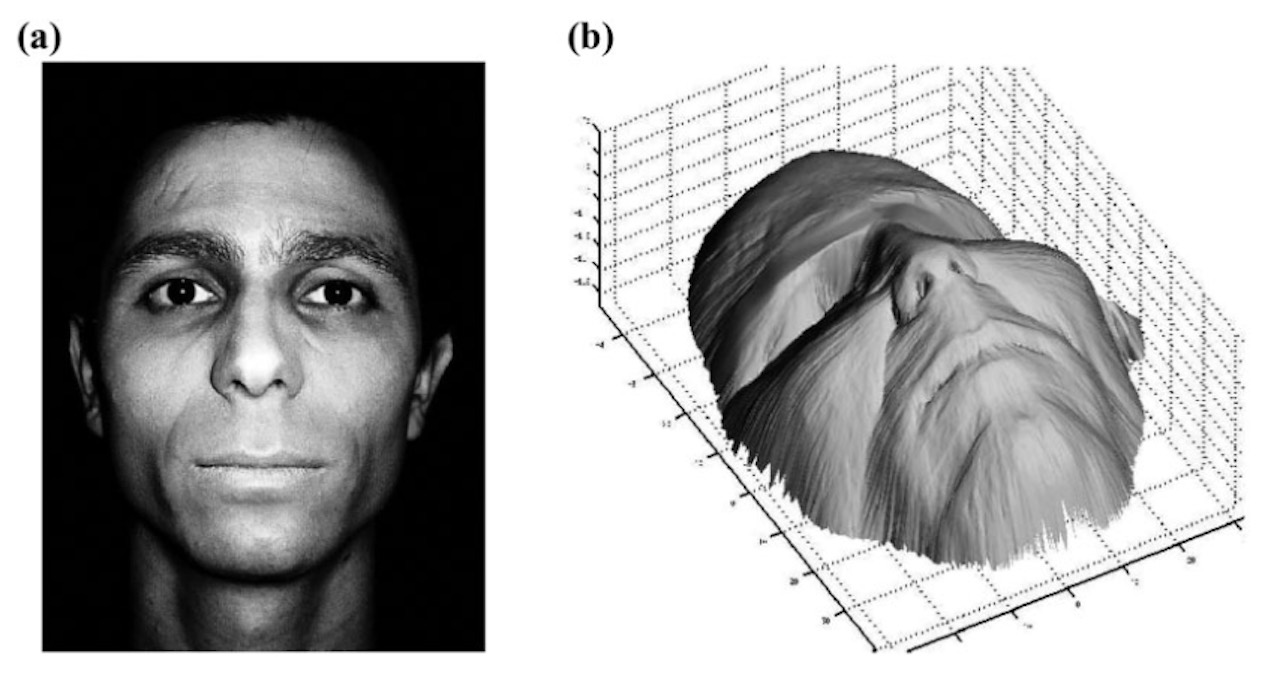
\includegraphics[width=0.5\linewidth]{images/shape_from_shading.jpg}
    \caption{Shape from shading \autocite{horn_shape_1989}}
    \label{fig:shape_from_shading}
\end{figure}

\subsection{Multi-view Stereo}
\textcite{furukawa_accurate_2010}

\subsection{Convolutional Neural Networks}
\textcite{krizhevsky_imagenet_2012}

\subsection{Voxel-based Approaches}
\textcite{zhirong_wu_3d_2015}

\subsection{Point Cloud-based Approaches}
\textcite{charles_pointnet_2017}
\subsection{Mesh-based Approaches}
\textcite{wang_pixel2mesh_2018}
\subsection{Neural Implicit Functions}

\textcite{park_deepsdf_2019}
\textcite{mildenhall_nerf_2021}

\section{Models}


\subsection{Models}
In the recent years several models have been developed to generate 3D models from 2D images. Some of the most prominent models include:
\subsubsection{One-2-3-45}
This model was developed by \textcite{liu_one-2-3-45_2023-1}...

\subsubsection{Zero-1-to-3}
Zero-1-to-3 is a model developed by \textcite{liu_zero-1--3_2023}...
\subsubsection{TripoSR}
TripoSR is a model developed by \textcite{tochilkin_triposr_2024}...

\subsection{Comparison}
Result comparison between models both visually and in terms of performance.

\section{Applications of 3D Mesh Reconstruction}
As the field is still relatively new, no mainstream applications have been established yet. However, the potential is great and some possible applications have already been identified.

\subsection{Development and Entertainment}
The most prominent application of 3D mesh reconstruction could be in the development and entertainment industry. The ability to generate 3D models from 2D images could revolutionize the asset creation process.
This could be especially beneficial for indie developers or small studios that do not have the resources to create high-quality 3D models from scratch. The generated models could be used in video games, movies, animations, and other forms of media. This could significantly reduce the time and cost associated with creating 3D assets, allowing developers and animators to focus on other aspects of their projects. (see Figure \ref{fig:one-2-3-4-5-plus-plus-demo})
\begin{figure}
    \centering
    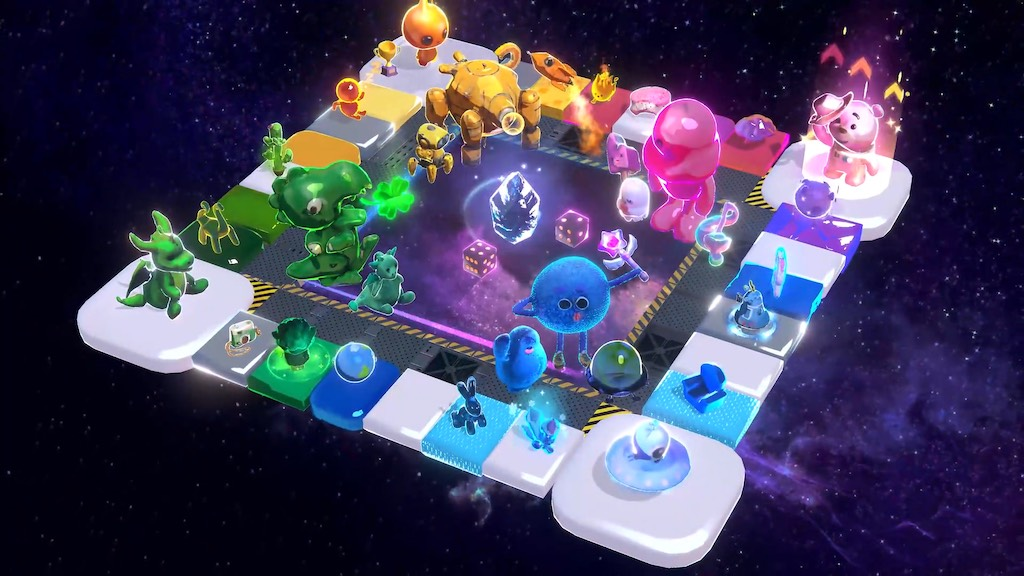
\includegraphics[width=1\linewidth]{images/one-2-3-45++_demo.jpg}
    \caption{Models generated by One-2-3-45++ \autocite{liu_one-2-3-45_2023-1}}
    \label{fig:one-2-3-4-5-plus-plus-demo}
\end{figure}

\subsection{Medical}

\subsection{Other Applications}

\subsubsection{Cultural Heritage}

% \section{Ethical Implications}
% Even though all the advancements in the field of 3D mesh reconstruction are promising, they also raise quite a few concerns.

% \subsection{Environmental Impact}
% Estimations of energy consumption for training as well as execution of models.

% \subsection{Training Data}
% The sources of training data. Looking at datasets like Objaverse-XL \autocite{deitke_objaverse-xl_2023} and their sources.

% \subsection{Privacy Concerns}

% \subsection{Cultural Sensitivity}
% It is important that the models are actually representative of the cultures, especially when generating models of people or culturally significant objects.

% \subsection{Implications of Estimations and Hallucinations}
% It is usually necessary for these models to estimate not seeable parts of the object. This can lead to hallucinations and other artifacts in the generated models.

% \section{Implementation}
% Provide implementation details such as the used software and our software architecture, highlight your own solutions to encountered difficulties. Describe relevant iterations of your implementation.

% Describe your methodology. How did you evaluate your work? Why did you choose this methodology? Present results of your evaluation here.

\section{Discussion and Future Direction}
Discussion of results and their implications. What are the limitations current works? What are the next steps in this research area?
% Discuss your results to answer your research question. Does your data support you hypotheses? Put your results into perspective by situating it in the research field/related work.

\section{Conclusion}
% Summarize your work, outline limitations and future work.

% \section{Formatierung}
% \label{section:Formatting}

% Text mit beliebigen Sonderzeichen in UTF-8 ohne BOM \ldots
% ,
% \textbf{hervorgehobener Text},
% \texttt{void}\footnote{Fußnote 1},
% mathematische Formel im Text $\sum_{i=0}^n i^2$
% \ldots

% Referenz auf Unterabschnitt \ref{subsection:Coding} der Arbeit, automatisch richtig nummeriert.

% \textcite[]{Mulloni:2010} für einen einen Literaturverweis im laufenden Text.

% Literaturverweise sind essentiell für eine wissenschafliche Arbeit. \autocite[]{McConnell:2004:CCS:1096143}.

% Achtung: nur zitierte Literatur wird im Literaturverzeichnis
% angeführt.\footnote{Fußnote 2}


% Wir verwenden \LaTeX\footnote{ \url{http://en.wikibooks.org/wiki/LaTeX}} -- und das
% ist keine Quelle, sondern blos eine URL.

% \subsection{Figures machen was sie wollen}

% % h = try to place the figure Here
% % t = try to place the figure at the Top of a page
% % p = try to place this figure along with others on a separate Page
% % Note that LaTeX has a sophisticated ranking algorithm to place figures.
% % It is not always easy to accept LaTeX's placing but it is harder doing it
% % manually. Just let it go ;-)
% \begin{figure}[!ht]
% 	\centering
% 	\subfloat[Das Julia Fraktal]{
% 		\includegraphics[width=0.75\linewidth]{images/Julia-Fractal.png}
% 		%for reference of this subfigure only
% 		\label{subfigure:Julia-Fractal}
% 	}
% 	\qquad
% 	\subfloat[Noise für Tinteneffekte]{
% 		\includegraphics[width=0.75\linewidth]{images/Perlin-Coherent.png}
% 		%for reference of this subfigure only
% 		\label{subfigure:Perlin-Coherent}
% 	}
% 	\caption[
% 		Verschiedene Pixelgraphiken\newline
% 		% source url given in the table of figures
% 		\small\texttt{https://mediacube.at/wiki/}
% 	]{
% 		Verschiedene Pixelgraphiken
% 	}
% 	%for reference to all subfigures
% 	\label{figure:PixelImages}
% \end{figure}

% Unterstützte Pixelgraphikformate: PNG, JPEG, PDF.
% Angabe von height oder width meist wichtig.

% Referenz auf Abbildung \ref{figure:PixelImages} mit allen Teilbildern.
% Referenz auf Unterabbildung \ref{subfigure:Julia-Fractal}.

% %figure* stretches figure over both columns
% \begin{figure*}[t]
% 	\centering
% 	\includegraphics[width=0.9\textwidth]{images/KappaGamma.pdf}
% 	\caption{
% 		Vektorgraphik mit \LaTeX\ Beschriftung ($\kappa$, $\gamma$)
% 	}
% 	%for reference to this figure
% 	\label{figure:KappaGammaTau}
% \end{figure*}

% Referenz auf Abbildung \ref{figure:KappaGammaTau}.

% Bei Vektorgraphik mit \LaTeX\ Beschriftung keine Skalierung mit width oder height verwenden.

% Vektorgraphik mit \LaTeX\ Beschriftung kann etwa mit \texttt{ipe} erstellt werden.

% Unterstütztes Vektorgraphikformat: PDF. EPS muss konvertiert werden.


% \subsection{Unterabschnitt 2}
% %for references to this subsection
% \label{subsection:Coding}

% \begin{listing}[H]
%     \begin{csharpcode*}{firstnumber=10}
%         while (true)
%         {
%             // Ignition
%         }
%     \end{csharpcode*}

%     \caption{Example of another listing.}
%     \label{lst:Main}
% \end{listing}

% Wie man in Listing \ref{lst:Main}, kann man die erste Zeilennummern im Listing absichtlich ändern, hier z.B. auf 10. Beachte, dass man hier chsarpcode* als Umgebung nutzt, um neben
% den Default-Settings zusätzliche Einstellungen zu tätigen.

% \subsubsection{Unterunterabschnitt i}

% Wörtliches Zitat:
% %select proper language if not in German
% \selectlanguage{english}
% \begin{quote}
% ``Erwin Unruh discovered that templates can be used to compute
% something at compile time. [...] The intriguing part of this exercise, however, was that the production of the prime numbers was performed by the compiler during the compilation process and not at run time.''

% \autocite[305]{Bosch2014}
% \end{quote}
% %select German again or the language that you were using before (note ngerman stands for New German)
% %\selectlanguage{ngerman}
% \selectthesislanguage


% \subsection{Unterabschnitt b}

% \begin{enumerate}
% 	\item Punkt 1
% 	\begin{enumerate}
% 		\item Unterpunkt 1
% 		\item Unterpunkt 2
% 	\end{enumerate}
% 	\item Punkt 2
% \end{enumerate}

% \begin{itemize}
% 	\item Punkt 1
% 	\begin{itemize}
% 		\item Unterpunkt 1
% 		\item Unterpunkt 2
% 	\end{itemize}
% 	\item Punkt 2
% \end{itemize}


% \subsection{Unterabschnitt c}

% \begin{table}[ht]
% 	\centering
% 	\begin{tabular}{r|rrr}
% 		    & $i$ & $j$ & $k$ \\ \hline
% 		$i$ &$-1$ & $k$ &$-j$ \\
% 		$j$ &$-k$ &$-1$ & $i$ \\
% 		$k$ & $j$ &$-i$ &$-1$
% 	\end{tabular}
% 	\caption{
% 		Multiplikationstabelle für Quaternionen
% 	}
% 	\label{table:Quaternions}
% \end{table}

% Referenz auf Tabelle \ref{table:Quaternions}.

% \section{Abschnitt 2}
% \label{section:MathematicalStuff}

% Sei $f(x)$ eine stetige Funktion, so ist die \textbf{Fourier Transformierte}
% $F(\omega)$ wie folgt definiert:
% \begin{equation}
% \label{equation:FourierDefinition}
% 	F(\omega) = \int_{-\infty}^{\infty} f(x) e^{-i\omega t} dt
% \end{equation}

% Referenz auf mathematische Gleichung (\ref{equation:FourierDefinition}).

% Unnummerierte Gleichung:
% \begin{equation*}
% 	e^{i\varphi} = \cos\varphi + i \sin\varphi
% \end{equation*}
% %you may also use \[ \] instead of \begin{equation*} and \end{equation*}

% Gleichungssystem:
% \begin{eqnarray}
% 	g(x) = f(x - x_0) & \Leftrightarrow &
% 		G(\omega) = F(\omega) e^{-i\omega x_0} \\
% 	g(x) = f(x) e^{i\omega_0 x} & \Leftrightarrow &
% 		G(\omega) = F(\omega - \omega_0)
% \end{eqnarray}
